\chapter{Kalman Filter}
If there is no uncertainty we can model our system as described in following picture:
\begin{figure}[!ht]
	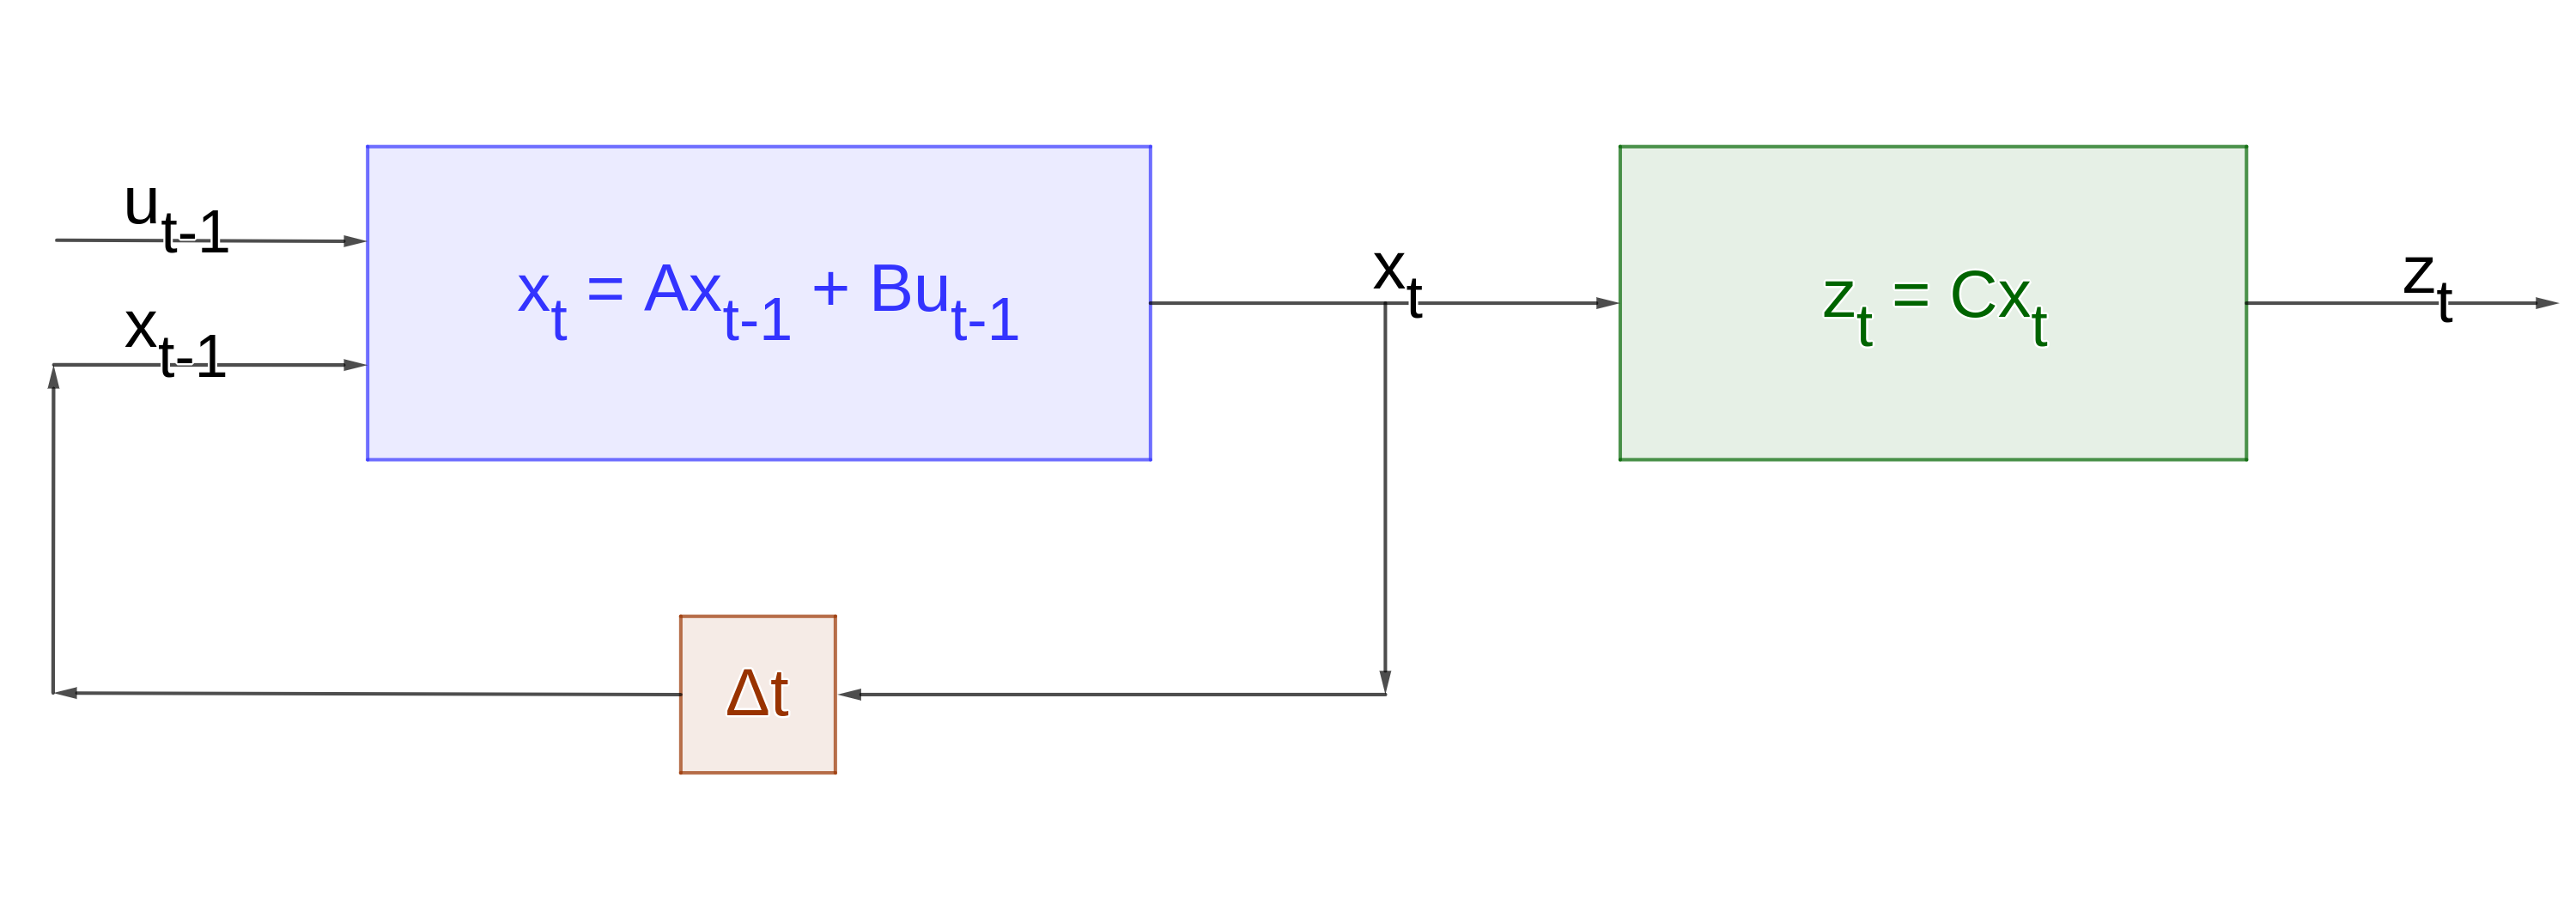
\includegraphics[scale=0.9]{system_model}
	\captionsetup{justification=centering, margin=1.5cm}
	\centering
	\caption{Deterministic System model.}
	\centering
\end{figure}
\begin{itemize}
	\item The state variables $x_t$ represents out robot's position and orientation.
	\item The control vector $u_t$ represents the rotational and translational accelerations our robot is subject to.
	\item The observation vector $z_t$ represents the sensors measurements.
\end{itemize}
As we can see in this model there is no uncertainty, the transition from a state to another is deterministic, we assume there is always no error in the observations or in the state.\\

However our inputs and our observations are not known with certainty. Therefore we must modify the previous model to include uncertainty and errors.
\begin{figure}[!ht]
	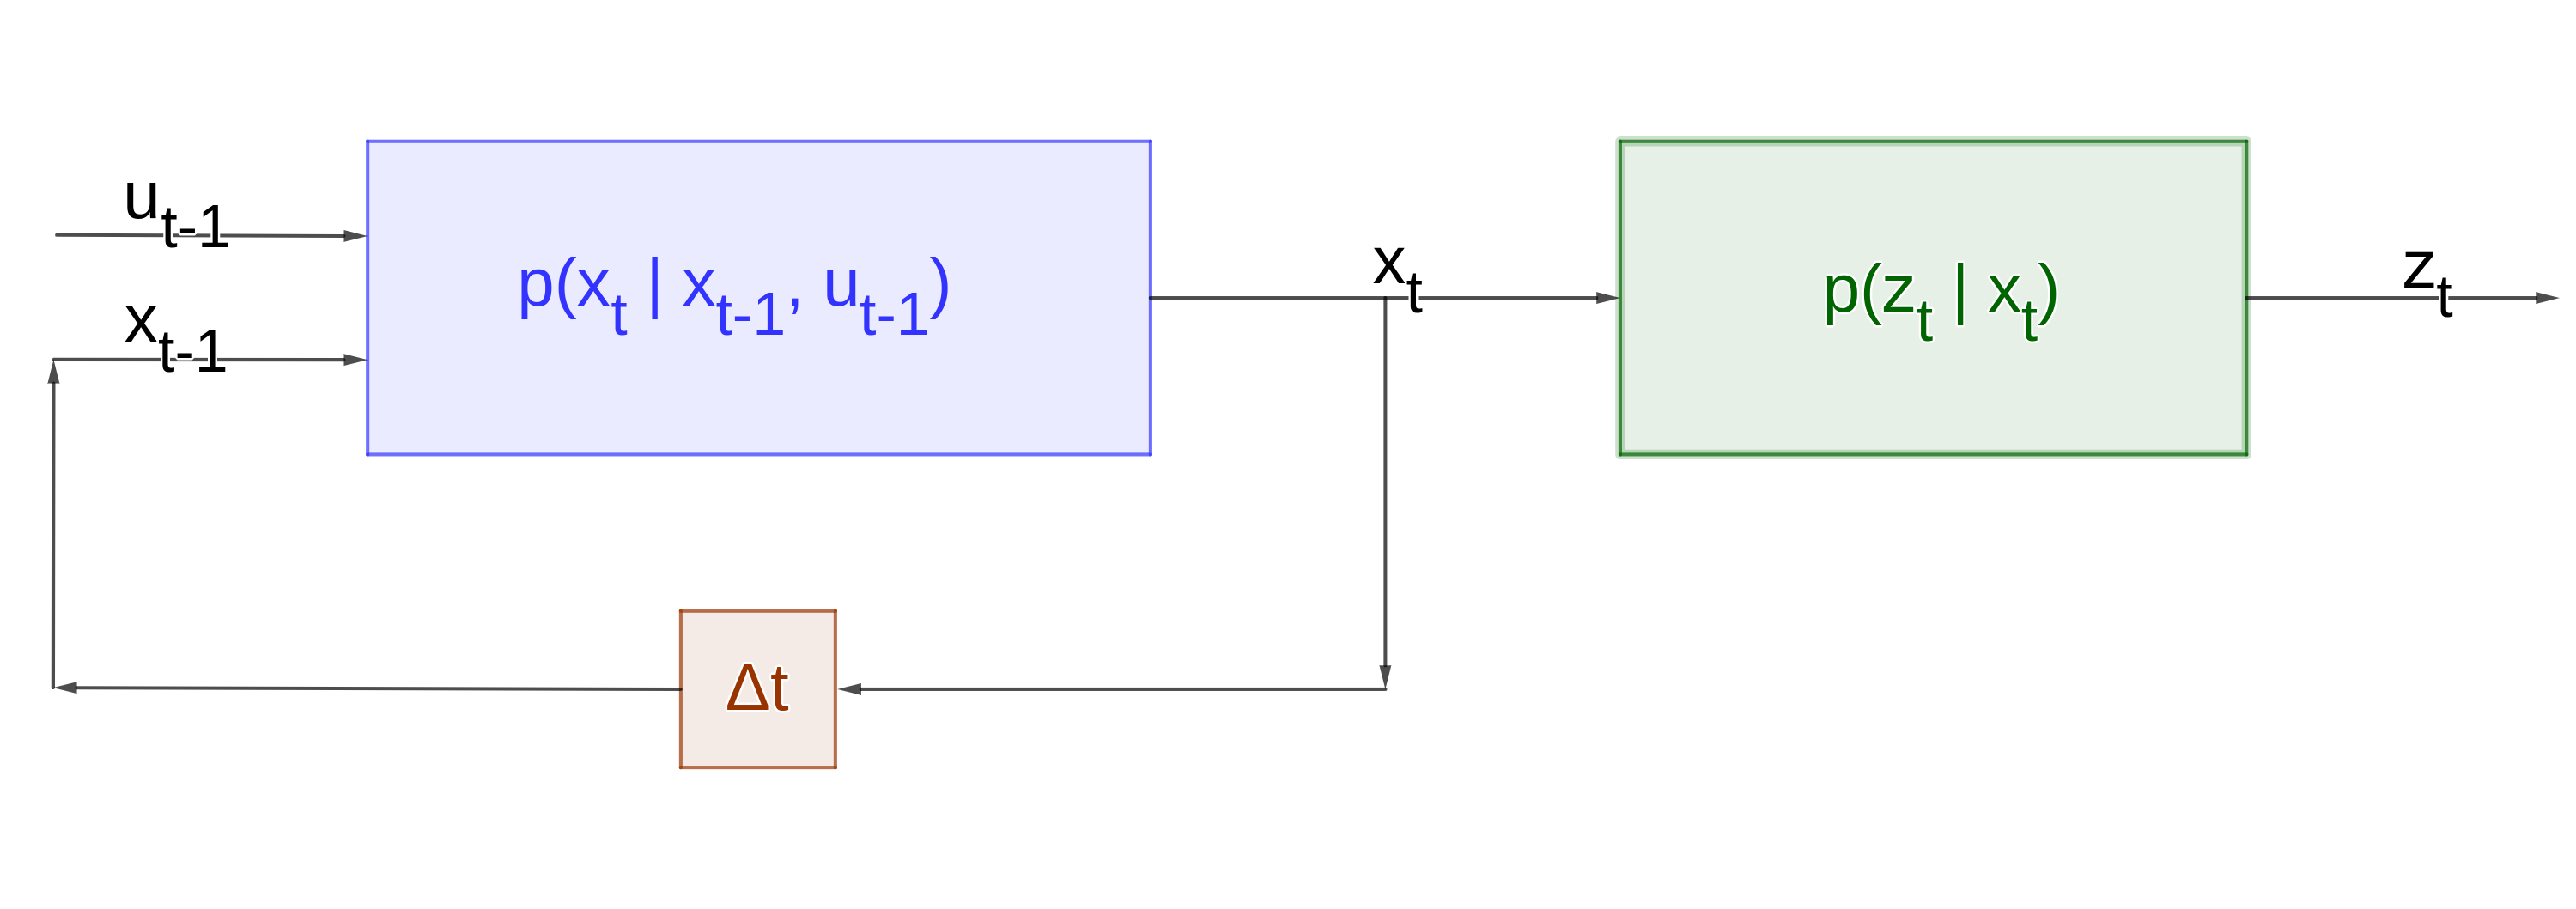
\includegraphics[scale=0.9]{stochastic_system_model}
	\captionsetup{justification=centering, margin=1.5cm}
	\centering
	\caption{Stochastic System model.}
	\centering
\end{figure}
\begin{itemize}
	\item $p(x_t | x_{t-1}, u_{t-1})$ is the transition model, which correlates the current state with the previous state and the previous control.
	\item $p(z_t | x_t)$ is the observation model, which correlates the current observation with the current state.
\end{itemize}

The goal of the Kalman filter is to compute the distribution over the current state given the sequence of all controls and of all observations up to the current instant, i.e. $p(x_t | u_{0:t-1}, z_{0:t})$.

As a basic idea we will perform two successive phases at each time instant, a predict phase and an update one.
\begin{itemize}
	\item In the predict phase we only consider the previous state and control to update the state. Therefore we will calculate the expected state in consequence to the control we gave to the system.
	\item In the update phase we update the state according to what we have observed and to how likely it is to have these observations from the current state.
\end{itemize}

In particular, in Kalman filtering we assume the state and the noise to be Gaussian. Since Gaussian distributions are closed under affine transformation, chain rule, marginalization and conditioning the state will always remain a Gaussian distribution. Therefore in each phase we will just have to compute the new parameters of the Gaussian.

In the following we will briefly present the Kalman filtering algorithm. For further details about Kalman Filtering we recommend the slides of the "Probabilistic Robotics" Course, held by Prof. Giorgio Grisetti at Sapienza University of Rome\supercite{prob_rob}.

\section{Predict phase}
In the predict phase we update the estimated state incorporating the latest control. The transition model is an affine transformation of the state and the control:
\begin{align}
	x_t = A_t x_{t-1} + B_t u_{t-1}\label{pred_model}
\end{align}
The previous state $x_{t-1}$ is a Gaussian with mean $\mu_{t-1|t-1}$ and covariance $\Sigma_{t-1|t-1}$.
While the control vector $u_{t-1}$ is a Gaussian with mean $\mu_{u,t-1}$ and covariance $\Sigma_{u,t-1}$.

After the predict phase, the estimated state $p(x_{t|t-1})$ is still a Gaussian, with the following parameters:
\begin{align}
	\mu_{t|t-1} &= A_t \mu_{t-1|t-1} + B_t \mu_{u,t-1}\label{pred_mean}\\
	\Sigma_{t|t-1} &= A_t \Sigma_{t-1|t-1} A_t^T + B_t \Sigma_{u,t-1} B_t^T\label{pred_cov}
\end{align}

\section{Update phase}
In the update phase we incorporate the new observations in the state estimate, starting form the observation model:
\begin{align}
	z_t = C_t x_{t|t-1}\label{upd_model}
\end{align}

We want to compute the probability $p(x_t|z_t)$ given the following distributions:
\begin{itemize}
	\item $p(z_t|x_t)$ which is a Gaussian distribution with mean $\mu_{z,t} = C_t x_{t|t-1}$ and covariance $\Sigma_{z,t}$,
	\item $p(x_{t|t-1})$ which is the Gaussian distribution of the estimated state after the predict phase.
\end{itemize}

In the update phase we compute the Kalman gain:
\begin{align}
	K_t = \Sigma_{t|t-1} C_t^T (\Sigma_{z,t} + C_t \Sigma_{t|t-1} C_t^T)^{-1}\label{kalman_gain}
\end{align}

Using the Kalman gain we can update the parameters of the Gaussian distribution representing the state:
\begin{align}
	\mu_{t|t} &= \mu_{t|t-1} + K_t (z_t - \mu_{z,t})\\
	\Sigma_{t|t} &= (I - K_t C_t) \Sigma_{t|t-1}
\end{align}

\paragraph{Role of the observation covariance}
We can rewrite the \ref{kalman_gain} as follows:
\begin{gather*}
	K_t = \frac{\Sigma_{t|t-1} C_t^T}{\Sigma_{z,t} + C_t \Sigma_{t|t-1} C_t^T}
\end{gather*}
In this form it becomes evident the role of the observation covariance $\Sigma_{z,t}$ in the update phase.\\

If the observation covariance (i.e. the observation uncertainty) tends to zero, then the Kalman Gain tends to:
\begin{gather*}
	K_t = \frac{\Sigma_{t|t-1} C_t^T}{C_t \Sigma_{t|t-1} C_t^T} = \frac{1}{C_t}	
\end{gather*}
and consequently:
\begin{align*}
	\mu_{t|t} &= \mu_{t|t-1} + K_t (z_t - \mu_{z,t}) = \mu_{t|t-1} + \frac{1}{C_t} (z_t - C_t \mu_{t|t-1}) =\nonumber\\
			&= \mu_{t|t-1} + \frac{1}{C_t} z_t - \mu_{t|t-1} = C_t^{-1}z_t\\
	\Sigma_{t|t} &= (I - K_t C_t) \Sigma_{t|t-1} = (I - \frac{1}{C_t} C_t) \Sigma_{t|t-1} = (I - I) \Sigma_{t|t-1} = 0
\end{align*}
Therefore if the observation uncertainty tends to zero, the state estimate can be calculated only from the current observation and will have zero covariance.\\

If the observation covariance tends to infinity, then the Kalman Gain tends to zero and consequently:
\begin{gather*}
	K_t = \frac{\Sigma_{t|t-1} C_t^T}{\Sigma_{z,t} + C_t \Sigma_{t|t-1} C_t^T} = 0
\end{gather*}
\begin{align*}
	\mu_{t|t} &= \mu_{t|t-1} + K_t (z_t - \mu_{z,t}) = \mu_{t|t-1}\\
	\Sigma_{t|t} &= (I - K_t C_t) \Sigma_{t|t-1} = \Sigma_{t|t-1}
\end{align*}
Therefore if the observation uncertainty tends to infinity, the state estimate will not be updated by the observations.\\

Wrapping up, if the observation covariance tends to zero, the state estimate will move immediately on the observations; while if the covariance tends to infinity the state estimate will not incorporate the observations.

